% mnras_template.tex 
%
% LaTeX template for creating an MNRAS paper
%
% v3.0 released 14 May 2015
% (version numbers match those of mnras.cls)
%
% Copyright (C) Royal Astronomical Society 2015
% Authors:
% Keith T. Smith (Royal Astronomical Society)

% Change log
%
% v3.2 July 2023
%	Updated guidance on use of amssymb package
% v3.0 May 2015
%    Renamed to match the new package name
%    Version number matches mnras.cls
%    A few minor tweaks to wording
% v1.0 September 2013
%    Beta testing only - never publicly released
%    First version: a simple (ish) template for creating an MNRAS paper

%%%%%%%%%%%%%%%%%%%%%%%%%%%%%%%%%%%%%%%%%%%%%%%%%%
% Basic setup. Most papers should leave these options alone.
\documentclass[fleqn,usenatbib]{mnras}

% MNRAS is set in Times font. If you don't have this installed (most LaTeX
% installations will be fine) or prefer the old Computer Modern fonts, comment
% out the following line

%\usepackage{newtxtext,newtxmath}
% Depending on your LaTeX fonts installation, you might get better results with one of these:
%\usepackage{mathptmx}
%\usepackage{txfonts}
% Use vector fonts, so it zooms properly in on-screen viewing software
% Don't change these lines unless you know what you are doing
\usepackage[T1]{fontenc}

% Allow "Thomas van Noord" and "Simon de Laguarde" and alike to be sorted by "N" and "L" etc. in the bibliography.
% Write the name in the bibliography as "\VAN{Noord}{Van}{van} Noord, Thomas"
\DeclareRobustCommand{\VAN}[3]{#2}
\let\VANthebibliography\thebibliography
\def\thebibliography{\DeclareRobustCommand{\VAN}[3]{##3}\VANthebibliography}


%%%%% AUTHORS - PLACE YOUR OWN PACKAGES HERE %%%%%

% Only include extra packages if you really need them. Avoid using amssymb if newtxmath is enabled, as these packages can cause conflicts. newtxmatch covers the same math symbols while producing a consistent Times New Roman font. Common packages are:
\usepackage{graphicx}	% Including figure files
\usepackage{amsmath}	% Advanced maths commands

%%%%%%%%%%%%%%%%%%%%%%%%%%%%%%%%%%%%%%%%%%%%%%%%%%

%%%%% AUTHORS - PLACE YOUR OWN COMMANDS HERE %%%%%

% Please keep new commands to a minimum, and use \newcommand not \def to avoid
% overwriting existing commands. Example:
%\newcommand{\pcm}{\,cm$^{-2}$}	% per cm-squared

%%%%%%%%%%%%%%%%%%%%%%%%%%%%%%%%%%%%%%%%%%%%%%%%%%

%%%%%%%%%%%%%%%%%%% TITLE PAGE %%%%%%%%%%%%%%%%%%%

% Title of the paper, and the short title which is used in the headers.
% Keep the title short and informative.
\title[Extragalactic Astronomy]{Balogh vs Dressler: Spectral classification}

% The list of authors, and the short list which is used in the headers.
% If you need two or more lines of authors, add an extra line using \newauthor
\author[Mary Verdugo]{
Mary Verdugo,$^{1}$\thanks{E-mail: mary.verdugo@userena.cl}
\\
% List of institutions
$^{1}$Estudiante de Magister en Astronomia, Universidad de La Serena\\
}

% These dates will be filled out by the publisher
\date{Mon, Dic 4}

% Enter the current year, for the copyright statements etc.
\pubyear{2023}

% Don't change these lines
\begin{document}
\label{firstpage}
\pagerange{\pageref{firstpage}--\pageref{lastpage}}
\maketitle

% Abstract of the paper


% Select between one and six entries from the list of approved keywords.
% Don't make up new ones.


%%%%%%%%%%%%%%%%%%%%%%%%%%%%%%%%%%%%%%%%%%%%%%%% %%

%%%%%%%%%%%%%%%%% BODY OF PAPER %%%%%%%%%%%%%%%%%%

\section{Spectral classification}

Follow the methods obtains from \citet[]{Balogh} with the data from
\citet[]{Dressler}, the aim of this essay is replicate the same figures
9 and 11 from the first paper mentioned with the data of the second, to understand how the classification of Balogh is better in fuction to separete between star forming and passive galaxies.
\\

\section{Methods}
One of the first thing that we do to understand the comparison between the two jobs, is to review the meta-data of the data to homogenize the tables. In the case of \citet{Dressler} we have: \textit{the EW of the $H\delta$  is negative when the line present \textbf{emission}} (see figure \ref{dresslertable}). In comparison, the description about this two line features in \citet{Balogh} is: \textit{... When the EW [O II] index is positive the line is in emission, while the EW $H\delta$ index is positive when the line is in \textbf{absorption}.}. This implies that the data for $H\delta$ from the \citet{Dressler} catalogue is the same in both catalogues,and [O II] needs to be multiplied by $-1$ to homogenize the data. Doing that, we replicate the fig. 9 and fig. 11 from the paper of \citet{Balogh} (see figure \ref{figsbaloghs}).
\\

Using a \texttt{python} libraries, we made the sames figures (see figure \ref{plotmio1} and figure \ref{plotmio2}) 

\begin{figure}
	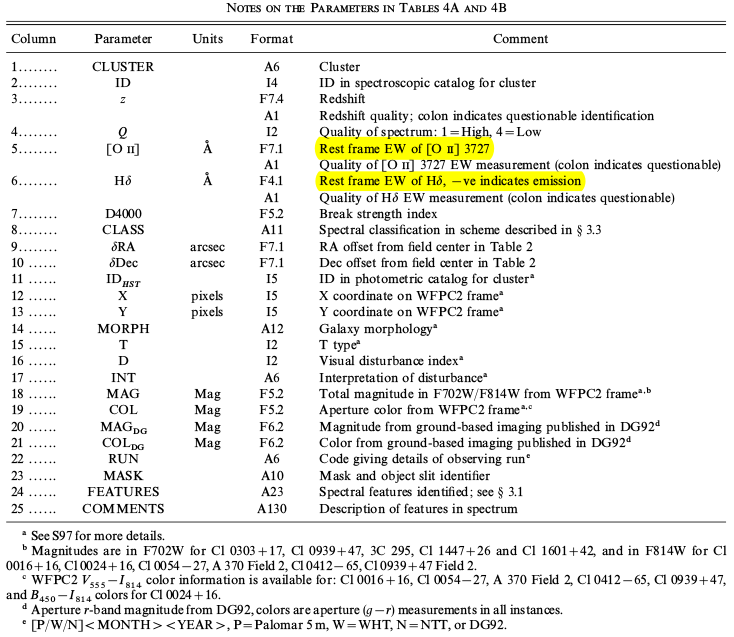
\includegraphics[width=\columnwidth]{/home/patito/Documents/egdatos/tableparameters.png}
    \caption{Capture of the table 5 from \citet{Dressler}}
    \label{dresslertable}
\end{figure}

\begin{figure}
	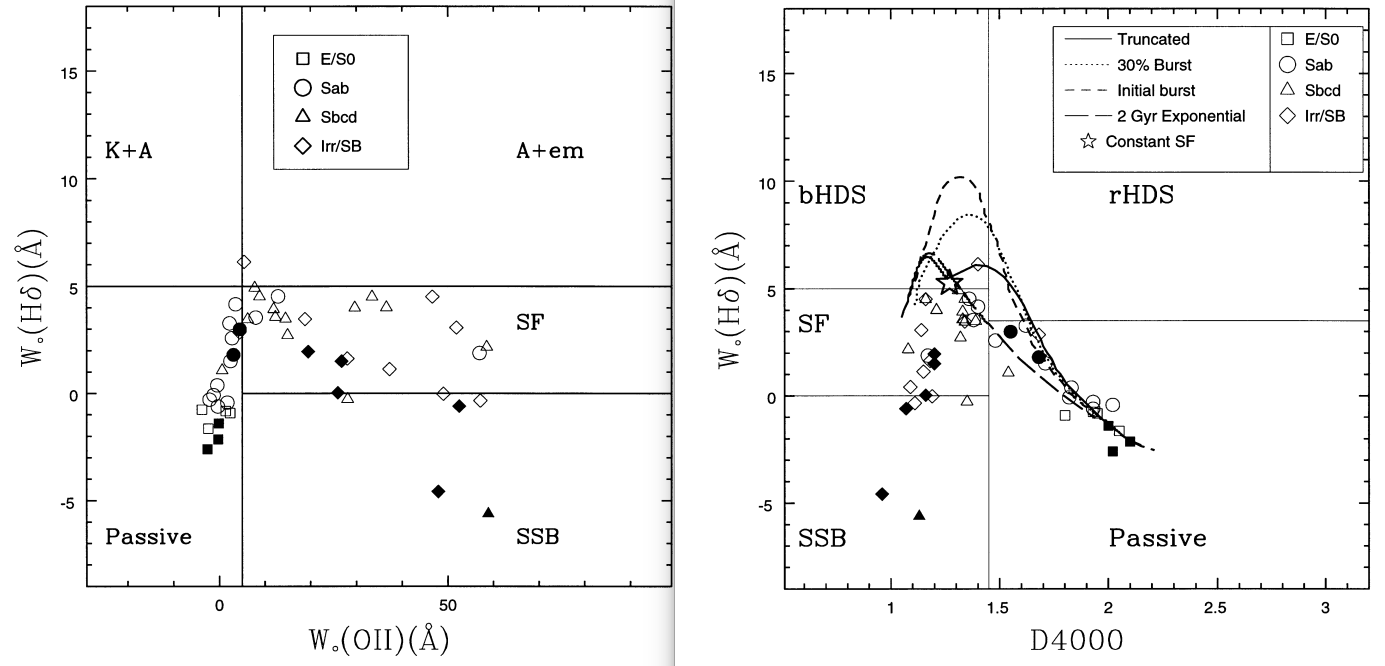
\includegraphics[width=\columnwidth]{/home/patito/Documents/egdatos/pdf/mnrastemplate/imagecomparison.png}
    \caption{figures 9 and 11 from the paper of \citet{Balogh}}
    \label{figsbaloghs}
\end{figure}

\begin{figure}
	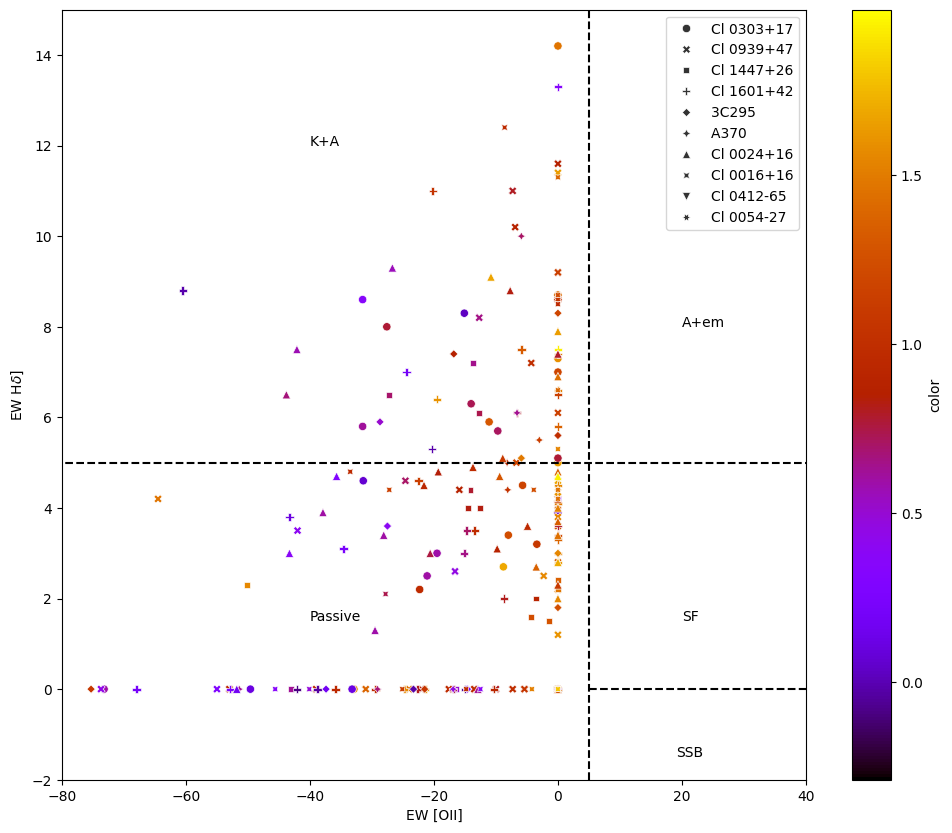
\includegraphics[width=\columnwidth]{//home/patito/Documents/egdatos/pdf/mnrastemplate/plotmio1.png}
	\caption{Figure made to replicate the first panel of the figure \ref{figsbaloghs}, this show the relation between the EW of $O[II]$ and EW of $H\delta$}
    \label{plotmio1}
\end{figure}

\begin{figure}
	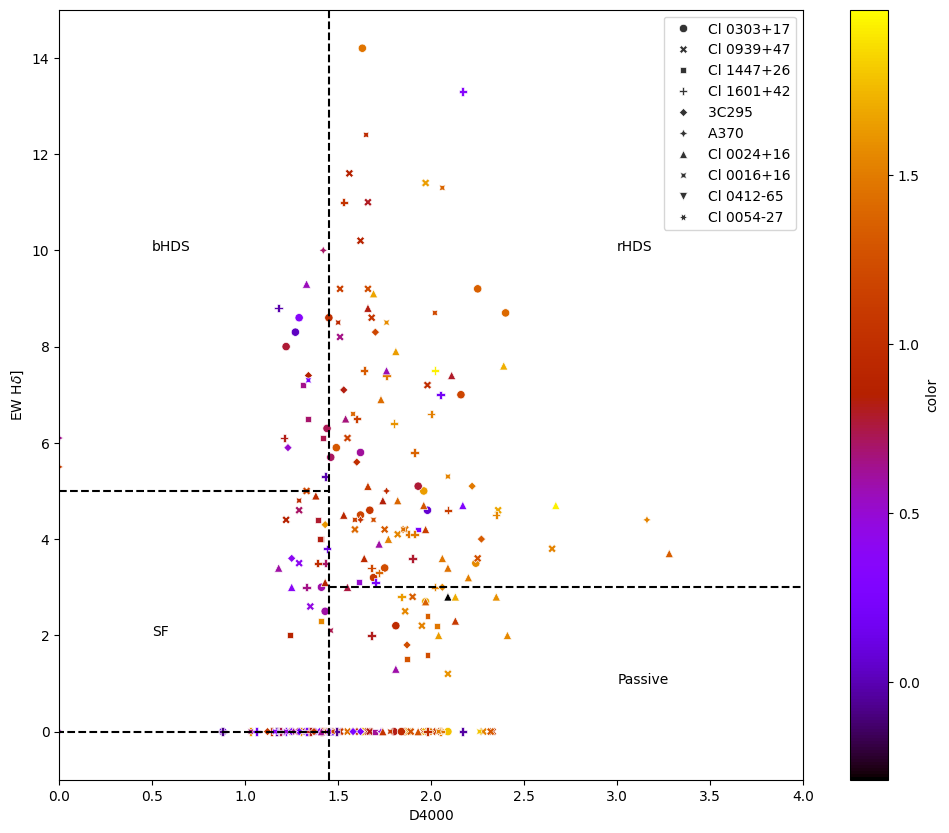
\includegraphics[width=\columnwidth]{//home/patito/Documents/egdatos/pdf/mnrastemplate/plotmio2.png}
	\caption{Figure made to replicate the second panel of the figure \ref{figsbaloghs}, this show the relation between the EW of $O[II]$ and EW of $H\delta$}
    \label{plotmio2}
\end{figure}

\begin{figure}
	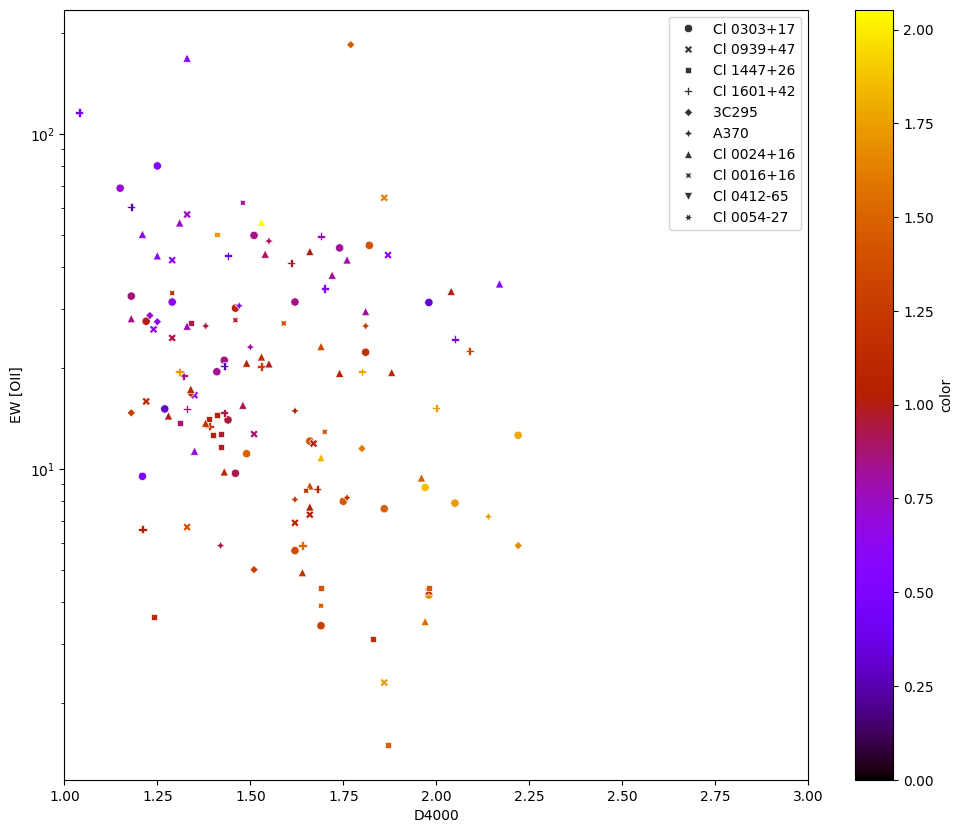
\includegraphics[width=\columnwidth]{//home/patito/Documents/egdatos/pdf/mnrastemplate/creacionpropia.png}
	\caption{This figure show the relation between EW of $O[II]$ vs D4000}
    \label{plotcreado}
\end{figure}


\begin{figure}
	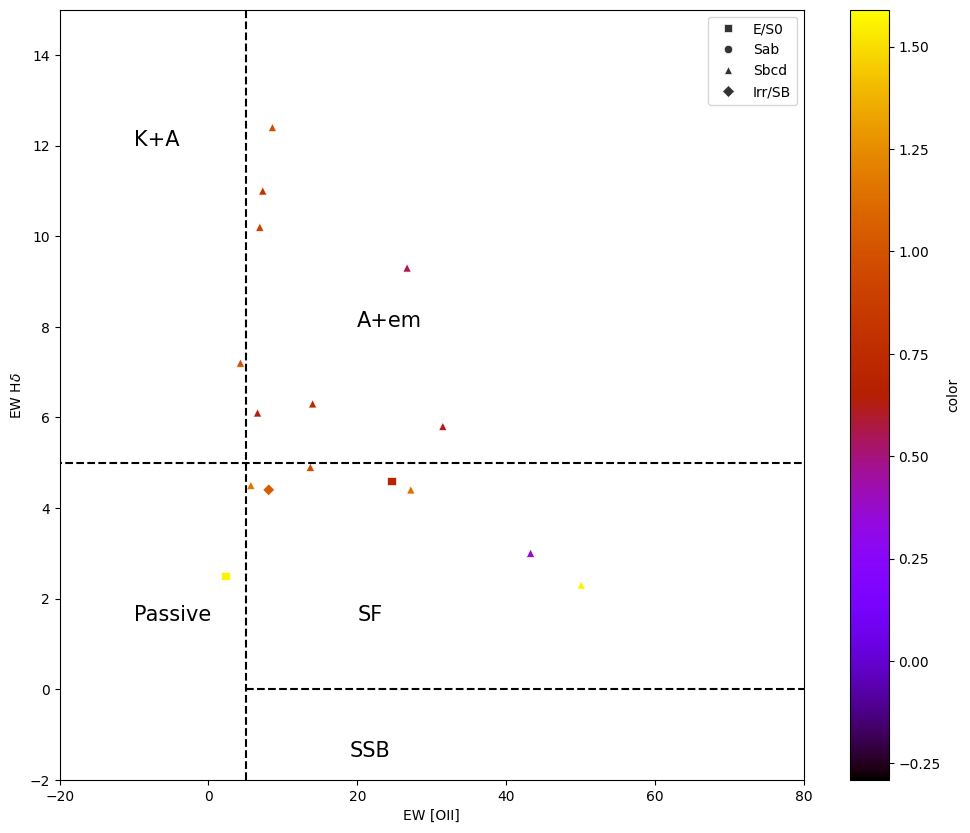
\includegraphics[width=\columnwidth]{///home/patito/Documents/egdatos/pdf/mnrastemplate/morfologicohdeltaoii.png}
	\caption{Figure to replicate the second panel of the figure \ref{figsbaloghs}, were replacing the morphology of the galaxies in function to have the sames of \citet{Balogh}}.
	\label{plotmorph1}
\end{figure}

\begin{figure}
	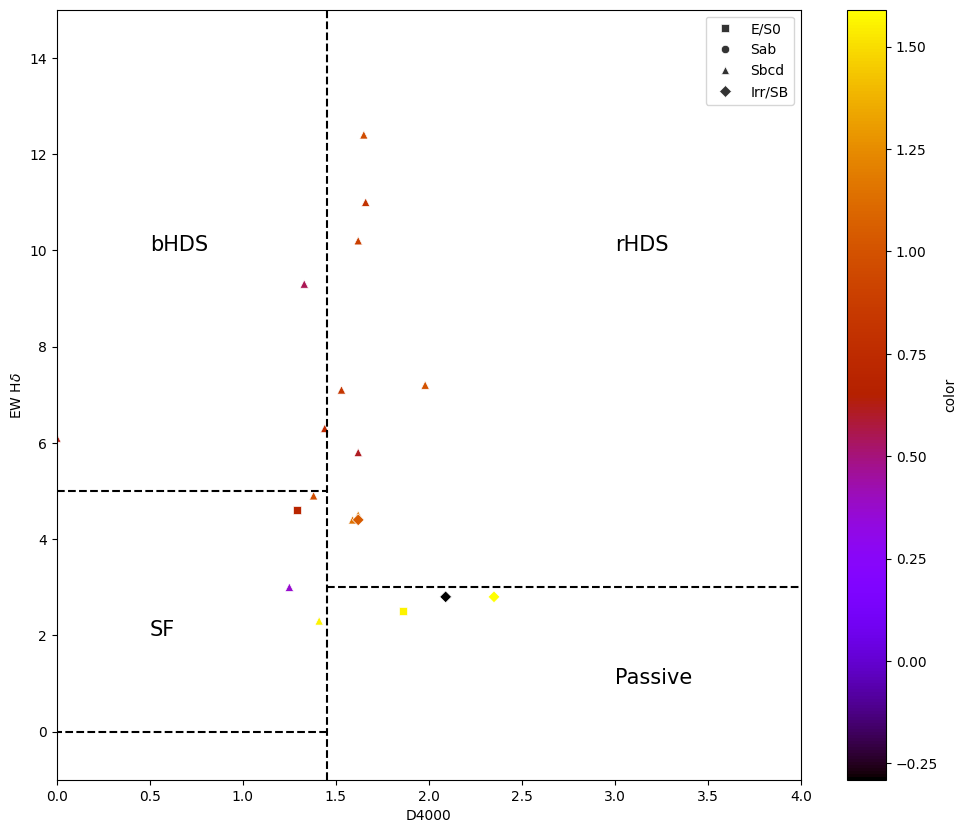
\includegraphics[width=\columnwidth]{//home/patito/Documents/egdatos/pdf/mnrastemplate/morfologicoHdeltad4000.png}
	\caption{Figure made to replicate the first panel of the figure \ref{figsbaloghs}, were replacing the morphology of the galaxies in function to have the sames of \citet{Balogh}}
	\label{plotmorph2}
\end{figure}

\begin{figure}
	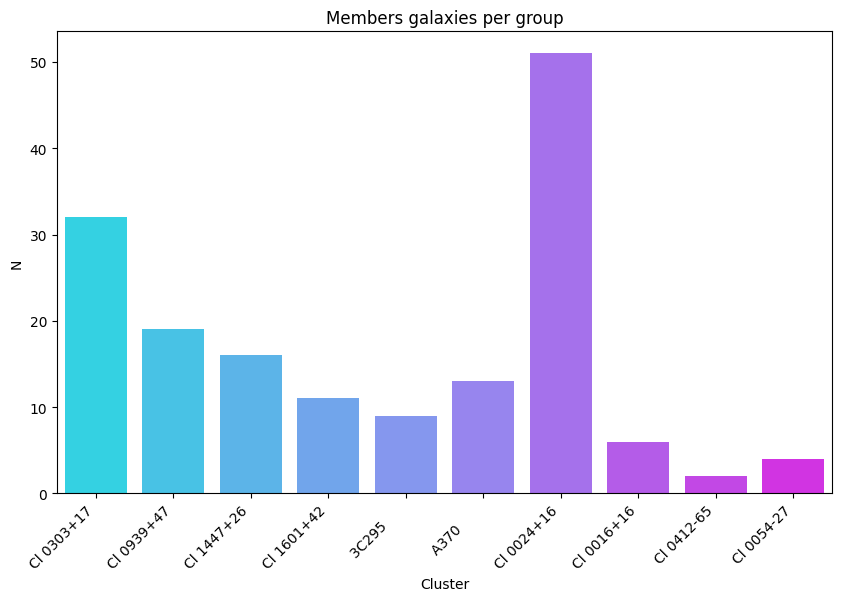
\includegraphics[width=\columnwidth]{//home/patito/Documents/egdatos/pdf/mnrastemplate/membergalaxies.png}
	\caption{Histogram for the count of galaxies per cluster}
	\label{histogram}
\end{figure}




\section{Analysis}
We made the sames graphics from \citet{Balogh} ussing the data provided by \citet{Dressler}, but with the aim to do the same morphological classification, we depure the data, excluding the galaxies from the \textit{field} and unified the morphological classification from \citet{Dressler}, i.e. we use the column of \textit{MType} in function to obtain \textit{E/S0, Sab, Sbcd, Irr/SB}, see figure \ref{plotmorph1} and \ref{plotmorph2}. And also, we made the plots separate by cluster. \\

In two cases, we can see a poorly stadistic. In order to confirm, we made the count of number of galaxies per cluster in the figure \ref{histogram}. It is important understand the context, this two papers was the first in the area of the spectral classification, but the data was be used carefully. \\

\subsection{H$\delta$ and the color}
H$\delta$ is an spectral line of absorption (Balmer's Series) related with the stars A and F. This line is strong in presence of recent star formation. So the EW H$\delta$ is a good indicator of recent star formation, and in relation to the color of the galaxies, is physically expected that the red galaxies has a low EW H$\delta$ and the blue galaxies show a high EW H$\delta$, but in the data there is not so evident in the figure \ref{plotmio1}. In the case of the figure \ref{plotmio2}, the relation of the color and H$\delta$ is more noticeable, but probably the relation with the color is for the D4000 parameter, that literally is related with the stellar continous of the galaxies, and this is related with the star formation history, i.e. the recent star formation. With this, we expected that the red galaxies show a high D4000 and the blue galaxies a low D4000, related with the age of the stellar populations. 

\subsection{O [II] and the color}
O[II] is an spectral line of emission with origin in the transition between energetic levels in the Oxygen atoms. In the context of the galaxies, this line be present when the young stellar populations (O, B stars) ionize the gas in the interstellar medium by their hot atmospheres, this is quickly related with the age of the star in a galaxy and we expected also, a high relation between the EW O[II] and the color of the galaxies, pointing to the color of the stellar populations. In this case we expected that the red galaxies has low or null EW O[II] and the blue galaxies has a high value for EW O[II]. The figure \ref{plotmio1}, show a correlation between the colors and the EW O[II], if we have a high EW O[II], the galaxies are more blue. 

\subsection{The classification}
To analyze the feature of the galaxies inside the "boxes" of classification, it is understood the physics concept behind, and the definitons are specified in \citet{Balogh}. But we can see, that the red galaxies are in agree with the Passive and K+A galaxies. In the case of the trnasition galaxies, that can be a "green" color galaxies, are distributed for all the data. The blues galaxies are related with the A+em and SF galaxies. The A+em galaxies can be related with dust-obscureced galaxies \citet{poggianti99} or related with the AGN in theirs nucleus. There is no galaxies in SSB. On the other hand, fig. \ref{plotmio2} reveals some inconsistencies regarding the color of galaxies  and the spectral classification according to the D4000 vs H$\delta$. This is particularly noticeable in galaxies classified as passive, which exhibit a very blue color. Additionally, it is expected by definition that rHDS galaxies are noticeably redder than bHDS galaxies. However, despite the presence of a slight trend in this behavior, there are also certain galaxies strongly blue in the rHDS zone and galaxies at the boundary between red and blue in the bHDS zone.

\subsection{D4000 vs O[II]}
Following the figure \ref{plotmio2}, we made the same plane using the data of the O[II] vs D4000 in the figure \ref{plotcreado}. Is natural think that the relation of the O[II] with the D4000 represent a proxy of the star formation history and the age of the stellar populations. We put the EW[OII] axis in logarithm to have a better visualization of the features. We can see a clear tendence for the blue galaxies to put in the top of the data, and the some red galaxies maybe dust-obscureced (\citet{poggianti99}). The red galaxies falling to the bottom of the data, and we can put a line to separete them (\ref{plotconlinea})




%%%%%%%%%%%%%%%%%%%% REFERENCES %%%%%%%%%%%%%%%%%%

% The best way to enter references is to use BibTeX:

\bibliographystyle{mnras}
\bibliography{example} % if your bibtex file is called example.bib


% Alternatively you could enter them by hand, like this:
% This method is tedious and prone to error if you have lots of references
%\begin{thebibliography}{99}
%\bibitem[\protect\citeauthoryear{Author}{2012}]{Author2012}
%Author A.~N., 2013, Journal of Improbable Astronomy, 1, 1
%\bibitem[\protect\citeauthoryear{Others}{2013}]{Others2013}
%Others S., 2012, Journal of Interesting Stuff, 17, 198
%\end{thebibliography}

%%%%%%%%%%%%%%%%%%%%%%%%%%%%%%%%%%%%%%%%%%%%%%%%%%

%%%%%%%%%%%%%%%%% APPENDICES %%%%%%%%%%%%%%%%%%%%%

% Don't change these lines
\bsp	% typesetting comment
\label{lastpage}
\end{document}

% End of mnras_template.tex
